\section{Auswertung}
\label{sec:Auswertung}

% \begin{figure}
%   \centering
%   \includegraphics{plots/plot.pdf}
%   \caption{Plot.}
%   \label{fig:plot}
% \end{figure}



% \begin{table}
%    % Notation :  {% nicht entfernen ist sehr wichtig sonst Fehler !!
% \parbox{0.48\textwidth}{% %Ermöglicht zwei Tabellen neben einander
%   \centering
%   \sisetup{round-mode = places , round-precision = 0,scientific-notation=fixed, fixed-exponent = 0}
%          %rundet Werte aus Stelle, Stelle = ,  macht einen bestimmten festen exponenten
%   \resizebox{\textwidth}{!}{%  % skaliert zu große Tabellen
%   \begin{tabular}{S@{${}\pm{}$} S} % fügt plus minus Fehler Schreibweise hinzu
%     \toprule
%      $\text{e}_b / \si{\milli\meter}$ &
%      $\text{d}_b /\si{\milli\meter} $ & $\text{f}_b / \si{\milli\meter} $\\
%     \midrule
%     \bottomrule
%   \end{tabular}
%   % }
%   \caption{Tabellenunterschrift}
%   \label{tab:tab}
% }
% % \end{table}
% % \begin{table}
% \parbox{0.48\textwidth}{%
%   \centering
%   \sisetup{round-mode = places , round-precision = 0,scientific-notation=fixed, fixed-exponent = 0}
%   % \resizebox{\textwidth}{!}{%
%   \begin{tabular}{S@{${}\pm{}$} S}
%     \toprule
%      $\text{e}_b / \si{\milli\meter}$ &
%      $\text{d}_b /\si{\milli\meter} $ & $\text{f}_b / \si{\milli\meter} $\\
%     \midrule
%     \bottomrule
%   \end{tabular}
%   % }
%   \caption{Tabellenunterschrift}
%   \label{tab:tab}
% }
% \end{table}
\subsection{Hysterese Kurve des Magnetfeldes}
Die Feldstärke $B$ wird gegen den Feldstrom $I$, in Abbildung \ref{fig:BFeldplot}, aufgetragen. 
Das ermöglicht später das Magnetfeld zu berechnen, bei dem die Aufspaltung der Spektrallinien 
zu beobachten ist. In der Abbildung wird durch den linearen Teil der aufsteigenden Hysteresekurve eine 
Ausgleichgerade gelegt. Die abfallende Hysteresekurve wurde zur Vollständigkeit gemessen und 
eingetragen. Die Ausgleichsrechnung wird mit Hilfe von \cite{scipy} und der Funktion
\begin{equation*}
B\left(I\right) = a \cdot I + b
\end{equation*}
durchgeführt.  Daraus ergibt sich $ a = \SI{61.7(4)}{\milli\tesla\per\ampere}$ und 
$ b = \SI{9(3)}{\milli\tesla}$. Die in Abbildung \ref{fig:BFeldplot} schwarz makierten Werte wurden 
in der Ausgleichsrechnung nicht betrachtet, da diese nicht mehr im linearen Teil der Hysteresekurve 
liegen.
\begin{figure}
  \centering
  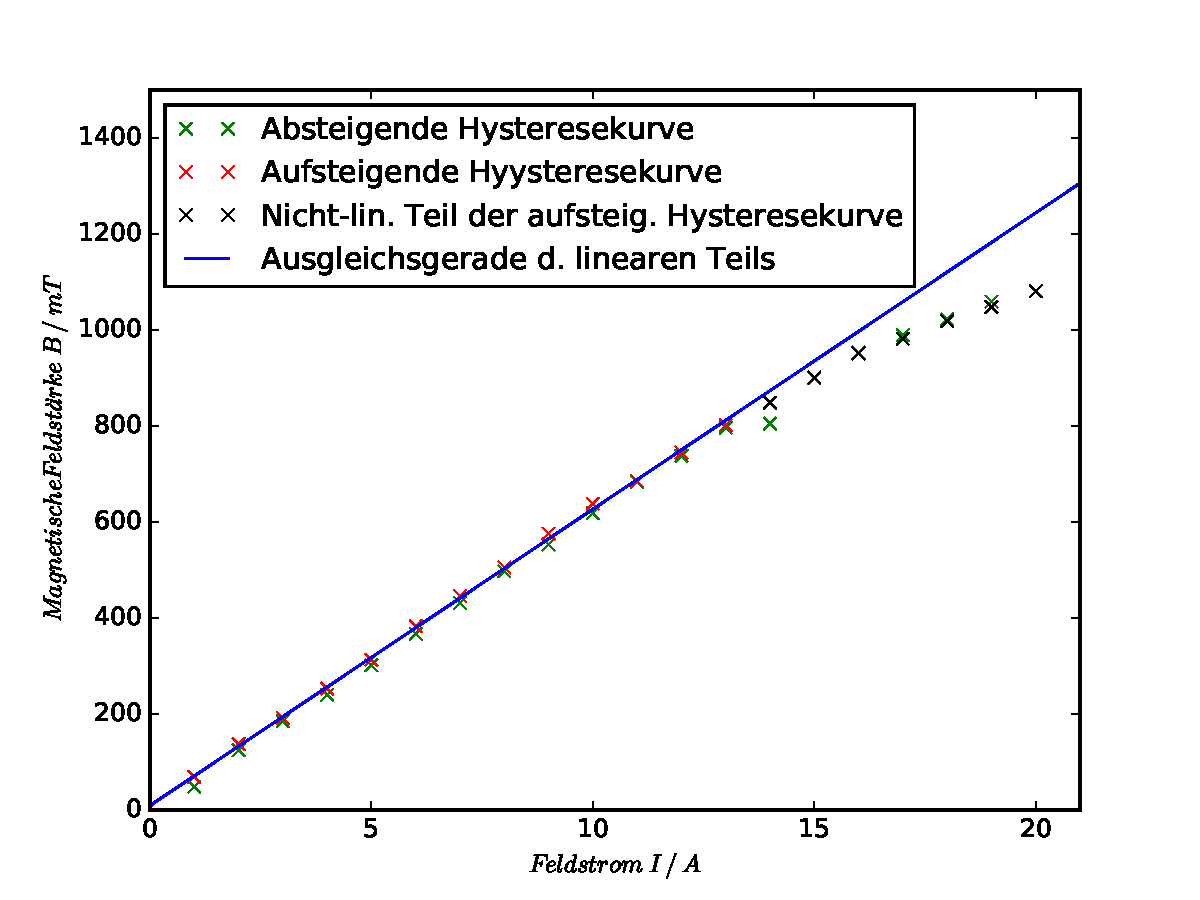
\includegraphics[height = 7cm]{plots/BFeldplot.pdf}
  \caption{Auf- und absteigende Hysterese Kurve des Magnetfeldes mit Ausgleichsgerade für den linearen Teil.}
   \label{fig:BFeldplot}
\end{figure}


\subsection{Methode zur Auswertung des Bildmaterials}

\subsection{Zeeman-Effekt beim Übergang von \texorpdfstring{${}^1\symup{P}_1 \iff {}^1 \symup{D}_2$}{math} in Cadmium}

\subsection{Zeeman-Effekt beim Übergang von \texorpdfstring{${}^3\symup{S}_1 \iff {}^3 \symup{P}_2$}{math} in Cadmium}
